\begin{figure}[t!]
  \centering
  \resizebox{\textwidth}{!}{%
  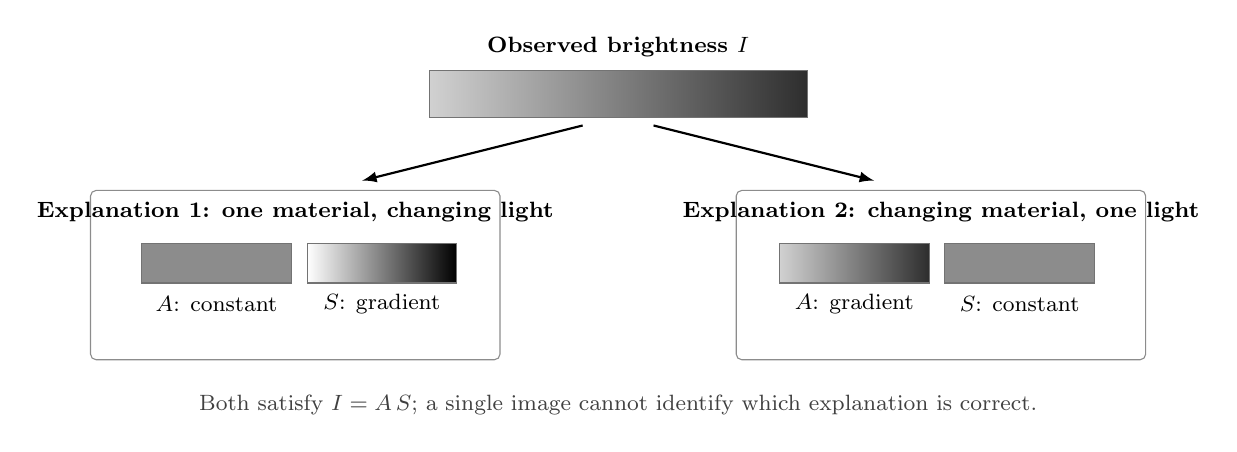
\begin{tikzpicture}[
    font=\small,
    >=latex,
    box/.style={draw=black!45, rounded corners=2pt, inner sep=7pt},
    lab/.style={font=\footnotesize\bfseries, align=center}
  ]
    \node[lab] at (0,1.55) {Observed brightness $I$};
    \shade[left color=black!18,right color=black!82,draw=black!55]
      (-2.4,0.65) rectangle (2.4,1.25);

    \node[box, minimum width=5.2cm, minimum height=2.15cm] at (-4.1,-1.35) {};
    \node[lab] at (-4.1,-0.55) {Explanation 1: one material, changing light};
    \fill[black!45,draw=black!55] (-6.05,-1.45) rectangle (-4.15,-0.95);
    \shade[left color=white,right color=black,draw=black!55]
      (-3.95,-1.45) rectangle (-2.05,-0.95);
    \node[font=\footnotesize] at (-5.1,-1.72) {$A$: constant};
    \node[font=\footnotesize] at (-3.0,-1.72) {$S$: gradient};

    \node[box, minimum width=5.2cm, minimum height=2.15cm] at (4.1,-1.35) {};
    \node[lab] at (4.1,-0.55) {Explanation 2: changing material, one light};
    \shade[left color=black!18,right color=black!82,draw=black!55]
      (2.05,-1.45) rectangle (3.95,-0.95);
    \fill[black!45,draw=black!55] (4.15,-1.45) rectangle (6.05,-0.95);
    \node[font=\footnotesize] at (3.0,-1.72) {$A$: gradient};
    \node[font=\footnotesize] at (5.1,-1.72) {$S$: constant};

    \draw[->,thick] (-0.45,0.55) -- (-3.25,-0.15);
    \draw[->,thick] (0.45,0.55) -- (3.25,-0.15);
    \node[font=\footnotesize,align=center,text=black!75] at (0,-3.0)
      {Both satisfy $I=A\,S$; a single image cannot identify which explanation is correct.};
  \end{tikzpicture}
  }
  \caption[Why intrinsic decomposition is ambiguous.]{%
    The intrinsic-image ambiguity in one dimension. The same observed brightness
    gradient can be explained by constant reflectance under changing illumination
    (left), or by changing reflectance under constant illumination (right).
    Retinex and learned IID methods resolve this underdetermined factorisation by
    adding spatial, semantic, and data-derived priors.
  }
  \label{fig:retinex_ambiguity}
\end{figure}
